% Created 2016-02-05 Fri 21:49
% Indented LaTeX compiler: pdflatex
\documentclass[aspectratio=169,presentation,bigger,fleqn,t]{beamer}
\usepackage[utf8]{inputenc}
\usepackage[T1]{fontenc}
\usepackage{graphicx}
\usepackage{grffile}
\usepackage{longtable}
\usepackage{wrapfig}
\usepackage{rotating}
\usepackage[normalem]{ulem}
\usepackage{amsmath}
\usepackage{textcomp}
\usepackage{amssymb}
\usepackage{capt-of}
\usepackage{hyperref}
\usetheme[titleformat=regular,numbering=none]{metropolis}
\setbeamerfont{frametitle}{shape=\upshape}
\usepackage{FiraSans}
\usepackage{setspace}
\setstretch{1.3}
\usepackage{booktabs}
\hypersetup{colorlinks=true,linkcolor=blue,urlcolor=blue}
\usetheme{default}
\author{John Henderson}
\date{2016 January (TCRUG meetup)}
\title{R + Org-mode = awesome!}
\subtitle{Org-mode for science, reproducible research, organization}
\hypersetup{
 pdfauthor={John Henderson},
 pdftitle={R + Org-mode = awesome!},
 pdfkeywords={},
 pdfsubject={},
 pdfcreator={Emacs 24.5.1 (Org mode 8.3.3)}, 
 pdflang={English}}
\begin{document}

\maketitle



\begin{frame}[fragile,label={sec:orgheadline1}]{Pre-warning}
 This presentation was \emph{a lot} harder than I thought it would be!
\begin{itemize}
\item Org-mode is great, but perhaps intimidating (emacs, setup\ldots{})
\item Emacs itself can be quite a barrier to entry
\item Background knowledge needed for feature \texttt{x} to make sense
\item There's a gazillion features I would love to talk about but can't
\end{itemize}
\end{frame}

\begin{frame}[label={sec:orgheadline2}]{My approach}
\begin{itemize}
\item Overview of some features
\item Demo of an Org file
\item Export with a few backends
\end{itemize}
\end{frame}


\begin{frame}[label={sec:orgheadline3}]{The life of a product developer}
Stuff I do in the course of my work (probably not that different from you!):

\begin{columns}
\begin{column}{0.5\columnwidth}
\begin{block}{Direct}
\begin{itemize}
\item write up experimental plans
\item do experiments
\item collect/analyze data
\item writeup reports/presentations
\item share/collaborate with others
\end{itemize}
\end{block}
\end{column}

\begin{column}{0.5\columnwidth}
\begin{block}{Indirect}
\begin{itemize}
\item record all sorts of info
\item meeting notes
\item manage todos
\item store contact info/notes
\item what to work on and when
\item emails
\end{itemize}
\end{block}
\end{column}
\end{columns}
\end{frame}

\begin{frame}[fragile,label={sec:orgheadline4}]{What the hell does emacs have to do with it?}
 Believe it or not, I \emph{learned Emacs} for \texttt{org-mode}. To date, it's the \emph{only} solution I'm
aware of that allows for all of the following in one place:
\begin{itemize}
\item notes
\item todos/time stamping/deadlines
\item tags/properties
\item embedded code + execution
\item export to multiple formats, with images, links, table of contents, automatically
generated code blocks and/or results\ldots{}
\end{itemize}

\pause

\emph{Pretty cool!}
\end{frame}

\begin{frame}[fragile,label={sec:orgheadline5}]{Some competition}
 I've always been a note taker, as I like to refer to the past\ldots{} you never know what
might be useful in the future! I tried all sorts of programs:

\begin{columns}
\begin{column}{0.5\columnwidth}
\begin{block}{recording work}
\begin{itemize}
\item Word/Writer
\item \href{http://zim-wiki.org/}{zim} (personal wiki)
\item \href{https://evernote.com/}{Evernote}
\item \href{http://tiddlywiki.com/}{TiddlyWiki}
\item \href{https://www.rstudio.com/}{RStudio}?
\end{itemize}
\end{block}
\end{column}


\begin{column}{0.5\columnwidth}
\begin{block}{Todos}
\begin{itemize}
\item \href{http://todotxt.com/}{\texttt{todo.txt}}
\item \href{https://en.wikipedia.org/wiki/Chandler_(software)}{Chandler}
\item \href{https://itunes.apple.com/us/app/igtd/id488595283?mt=8}{iGTD}
\item \href{http://tiddlywiki.com/}{TiddlyWiki}
\item \href{http://www.getontracks.org/}{tracks}
\end{itemize}
\end{block}
\end{column}
\end{columns}
\end{frame}

\begin{frame}[fragile,label={sec:orgheadline6}]{Ok, so what is it?}
 \texttt{Org-mode} is a major mode for the Emacs text editor.
\begin{itemize}
\item it uses markup to allow for structuring
\end{itemize}

\begin{verbatim}
* ok, so what is it?                          # heading

=Org-mode= is a major mode for the Emacs text editor.
- it uses markup to allow for structuring     # list
\end{verbatim}
\end{frame}

\begin{frame}[label={sec:orgheadline7}]{Markup}
\begin{block}{heading}
\begin{block}{subheading}
\begin{itemize}
\item unordered list
\end{itemize}


\begin{enumerate}
\item ordered list
\end{enumerate}


\alert{bold}, \emph{italic}, \uline{underline}, footnote \(\footnote[frame]{Footnote goes here}\),
superscripts\(^{\text{x}}\) and subscripts\(_{\text{y}}\), \href{https://www.google.com}{link}
\end{block}
\end{block}
\end{frame}

\begin{frame}[fragile,label={sec:orgheadline8}]{Markup}
 \begin{verbatim}
* heading
** subheading
- unordered list
1. ordered list
*bold*, /italic/, _underline_, footnotes[fn:1],
superscripts^x and subscripts_y,  [[https://www.google.com][link]] 

* Footnotes
Footnote goes here [fn:1]
\end{verbatim}
\end{frame}

\begin{frame}[label={sec:orgheadline9}]{Todos}
\begin{block}{do something}
\end{block}
\begin{block}{[1/2] meta task}
\begin{itemize}
\item $\boxtimes$ thing 1
\item $\square$ thing 2
\end{itemize}
\end{block}
\begin{block}{another thing}
\end{block}
\end{frame}

\begin{frame}[fragile,label={sec:orgheadline10}]{Todos}
 \begin{verbatim}
** todo do something
** todo [1/2] meta task 					       :proj:
   - [X] thing 1
   - [ ] thing 2
** done another thing
\end{verbatim}
\end{frame}

\begin{frame}[label={sec:orgheadline11}]{Time stamps}
Can add further information to notes (logs, deadlines, etc.)

\begin{block}{Notes about meeting with Dude}
\textit{[2016-01-18 Mon]}

Did blah blah blah
\end{block}

\begin{block}{do something}
\end{block}
\end{frame}


\begin{frame}[fragile,label={sec:orgheadline12}]{Time stamps}
 Can add further information to notes (logs, deadlines, etc.)

\begin{verbatim}
** Notes about meeting with Dude
[2016-01-18 Mon]

Did blah blah blah

** todo do something
   DEADLINE: <2016-01-21 Thu>
\end{verbatim}
\end{frame}


\begin{frame}[fragile,label={sec:orgheadline13}]{Tables/spreadsheet!}
 \begin{itemize}
\item Formulas: \texttt{\$} refers to column; \texttt{@} refers to row
\item Emacs \texttt{calc} has format specifiers built in
\end{itemize}

\begin{center}
\label{tab:orgtable1}

\begin{tabular}{lrr}
\toprule
id & x & y\\
\midrule
a & 2 & 1.33\\
b & 4 & 5.33\\
c & 6 & 12.00\\
\bottomrule
\end{tabular}
\end{center}
\end{frame}

\begin{frame}[fragile,label={sec:orgheadline14}]{Tables/spreadsheet!}
 \begin{verbatim}
#+tblname: dat_1
| *id* | *x* | *y* |
|------+-----+-----|
| a    |   2 |   4 |
| b    |   4 |  16 |
| c    |   6 |  36 |
#+TBLFM: $3=$2^2/3; %.2f
\end{verbatim}
\end{frame}

\begin{frame}[fragile,label={sec:orgheadline15}]{Inline code}
 I had \texttt{10} apples and I ate \texttt{4}. I must
have \texttt{6} left.
\end{frame}

\begin{frame}[fragile,label={sec:orgheadline16}]{Inline source code}
 \begin{verbatim}
I had src_R[:session r]{x <- 10; x} apples and I
ate src_R[:session r]{y <- 4; y}. I must have
src_R[:session r]{x - y} left.
\end{verbatim}
\end{frame}


\begin{frame}[fragile,label={sec:orgheadline17}]{Source blocks}
 \begin{verbatim}
#+name: code-ex1
#+header: data = dat_1
#+begin_src R :session r :exports results :results output

library(ggplot2)
sum(data$y)

#+end_src
\end{verbatim}

\begin{verbatim}
[1] 18.66
\end{verbatim}
\end{frame}


\begin{frame}[fragile,label={sec:orgheadline18}]{Plotting}
 \begin{verbatim}
p <- ggplot(data, aes(x = x, y = y, colour = id))
p + geom_point(size = 4) + theme_bw()
\end{verbatim}

\begin{center}
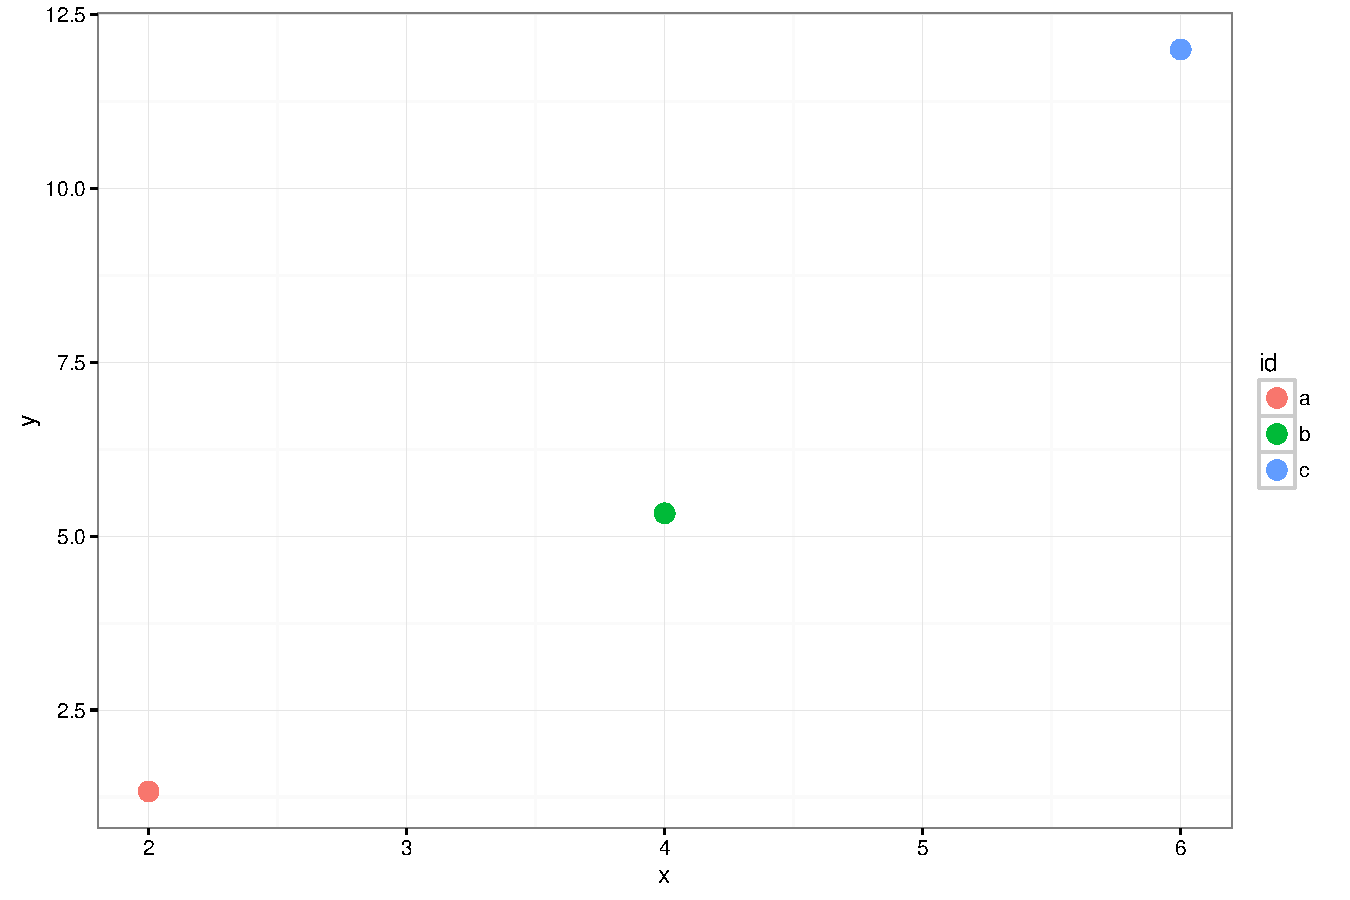
\includegraphics[height=5cm]{./plots/dat1_scatter.pdf}
\end{center}
\end{frame}

\begin{frame}[fragile,label={sec:orgheadline19}]{Plotting}
 \begin{verbatim}
#+name: dat1_plot
#+header: :var data = dat_1 :file ./plots/dat1_scatter.pdf
#+header: :width 9 :height 6
#+begin_src R :session r :exports both :results output graphics

p <- ggplot(data, aes(x = x, y = y, colour = id))
p + geom_point(size = 4) + theme_bw()

#+end_src
\end{verbatim}
\end{frame}

\begin{frame}[fragile,label={sec:orgheadline20}]{Formatting results}
 \begin{verbatim}
#+begin_center
#+attr_latex: :height 5cm
#+RESULTS: dat1_plot
[[file:./plots/dat1_scatter.pdf]]
#+end_center
\end{verbatim}
\end{frame}

\begin{frame}[fragile,label={sec:orgheadline21}]{Agenda}
 Like a search engine for your files
\begin{itemize}
\item Extracts todos, time stamps, tags, etc.
\item Can apply filters (keywords + the above)
\item Create custom views (only todo keyword \texttt{x})
\end{itemize}
\end{frame}


\begin{frame}[label={sec:orgheadline22}]{}
\vspace{0.4\textheight}

\begin{center}
Demo time!
\end{center}
\end{frame}

\begin{frame}[label={sec:orgheadline23}]{Some tips}
If you find this intriguing but intimidating, start small
\begin{itemize}
\item Start journaling in Org
\item Track todos
\item Edit a text file in Emacs
\item Create one document via export
\item Only customize and learn new features as needed
\end{itemize}


Ask for help
\begin{itemize}
\item The mailing list is awesome!
\item SO has quite a few Org questions
\end{itemize}
\end{frame}

\begin{frame}[fragile,label={sec:orgheadline24}]{Extra stuff}
 \begin{itemize}
\item Manage contacts with \href{https://julien.danjou.info/projects/emacs-packages#org-contacts}{org-contacts}
\item Text based file manager: \href{http://www.emacswiki.org/emacs/Sunrise_Commander}{Sunrise Commander}
\item A \href{http://www.gnu.org/software/emacs/tour/}{tour of Emacs}
\item \href{http://www.taskjuggler.org/}{Taskjuggler}, an Org-mode compatible project planner
\item Draw in \LaTeX with \href{http://www.texample.net/tikz/}{TikZ/pgf}
\item Beamer \href{https://github.com/matze/mtheme}{metropolis theme} (beamer that doesn't look like it)
\item Using \texttt{git} (\href{http://www.emacswiki.org/emacs/Git}{Emacs wiki} and \href{https://github.com/magit/magit}{magit}, a pretty popular tool)
\end{itemize}
\end{frame}

\begin{frame}[label={sec:orgheadline25}]{Learning Org}
\begin{itemize}
\item Org-mode manual: \url{http://orgmode.org/manual/}
\item Worg, the Org-mode wiki: \url{http://orgmode.org/worg/}
\item Org-mode mailing lsit: \url{http://orgmode.org/community.html}
\item Compact Org-mode guide: \url{http://orgmode.org/guide/}
\item Org-mode shortcut reference card: \url{http://orgmode.org/orgcard.pdf}
\item Brent Hanson's personal collection of settings, tips, and tricks: \url{http://doc.norang.ca/org-mode.html}
\end{itemize}
\end{frame}

\begin{frame}[label={sec:orgheadline26}]{References}
\begin{itemize}
\item Schulte, Eric; Davison, Dan; Dye, Thomas S; Dominik, Carsten. \emph{A Multi-Language Computing Environment for Literate Programming and Reproducible Research}. 
Journal of Statistical Software. \url{http://www.jstatsoft.org/article/view/v046i03}

\item Dye, Thomas S. \emph{Structure and Growth of the Leeward Kohala Field System: An
Analysis with Directed Graphs}. PlosONE. \url{http://journals.plos.org/plosone/article?id=10.1371/journal.pone.0102431}
\end{itemize}
\end{frame}
\begin{frame}[label={sec:orgheadline27}]{Examples}
\begin{itemize}
\item \href{https://github.com/jwhendy/devFest-shiny_2015}{2015 Google Developer Fest presentation}
\item \href{https://github.com/jwhendy/devFest-geo}{2014 Google Developer Fest presentation}
\item \href{https://drive.google.com/open?id=0BzQupOSnvw08anh6c3FwaGlHWVk}{Hobby analysis of a multi-level marketing company}
\end{itemize}
\end{frame}
\begin{frame}[label={sec:orgheadline28}]{the plot}
\begin{center}
\begin{figure}[htb]
\centering
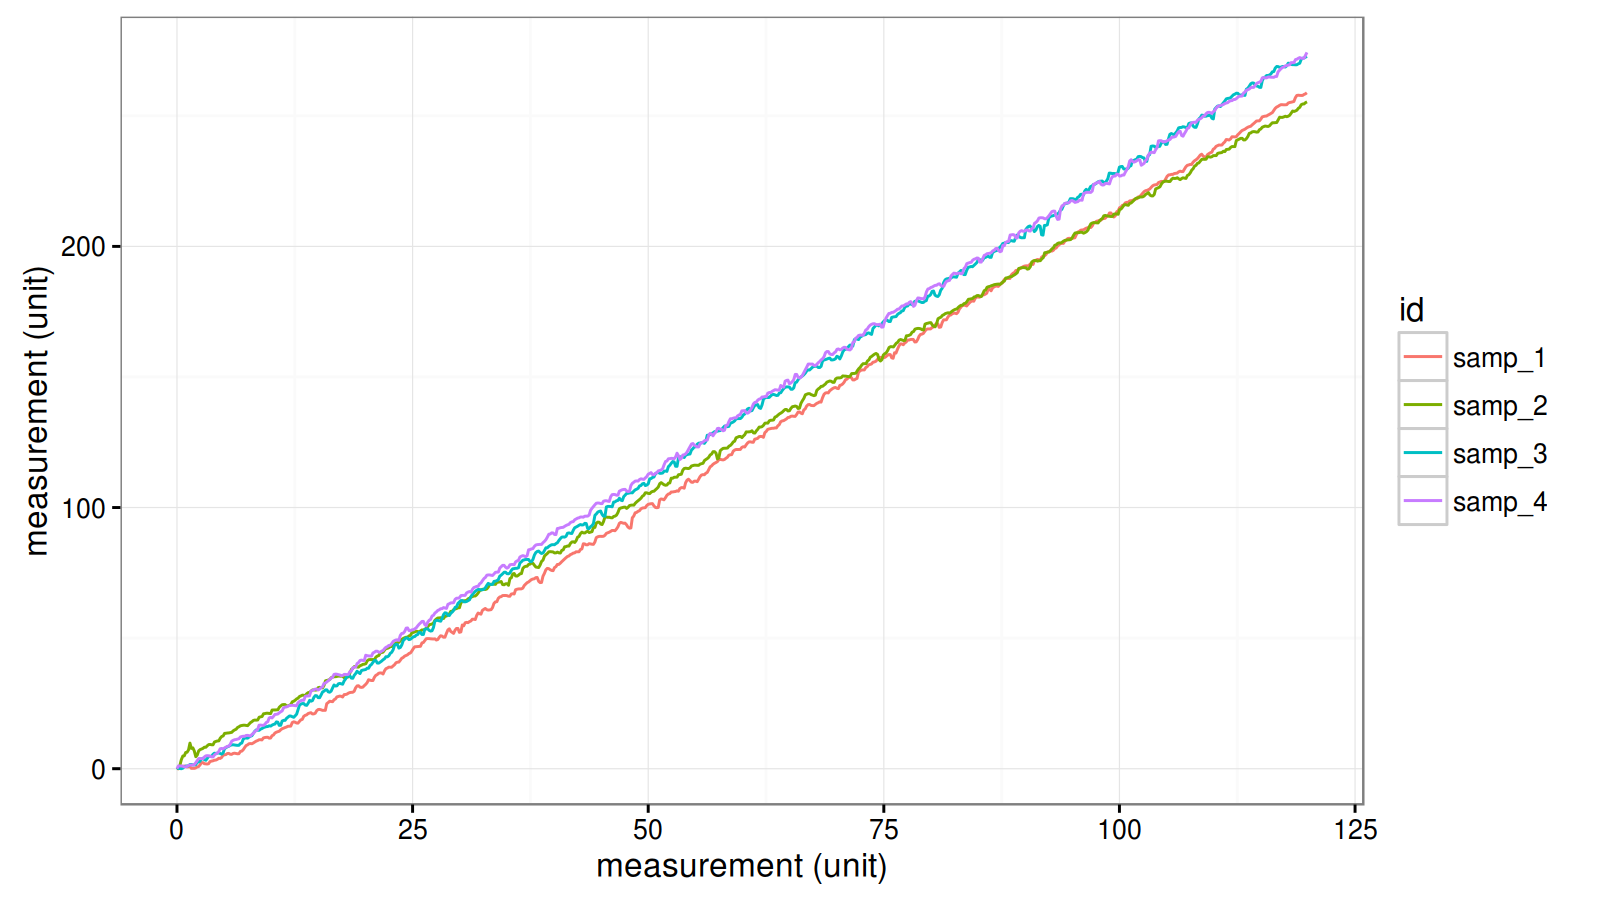
\includegraphics[width=0.9\textwidth]{./demo/plots/rate-comparison.png}
\caption{Rate comparison of samples 1-4}
\end{figure}
\end{center}
\end{frame}
\end{document}
